This chapter describes the search for a neutral MSSM Higgs boson through its decay to a pair of hadronically decaying tau leptons ($H \rightarrow \tauh\tauh$). Both CMS and ATLAS collaborations have discovered a Higgs boson's direct decay into a pair of $\tau$ \cite{ATLASHtt,CMSHtt}. In the context of the MSSM, three neutral Higgs bosons are predicted: the CP-even states h and H and the CP-odd state A, which may all decay to $\tau$ pairs. The search is performed in the $m_A - \mathrm{tan}\beta$ parameter space of the $m_{h}^{max}$ scenario \cite{Carena2003} for $m_A$ in the range 90 GeV to 3200 GeV. The analysis is sensitive to production via gluon-gluon fusion and production in association with b-quarks. The cross section of the latter increases for larger values of $\mathrm{tan}\beta$ due to the enhanced down-type fermion Yukawa couplings. A model-independant search for a single Higgs boson, denoted $\Phi$, is performed in the same mass range.

Searches for MSSM neutral Higgs bosons have been performed by the collaborations at LEP \cite{Schael2006}, the Tevatron \cite{Benjamin:2010xb}, and at LHC by the CMS and ATLAS collaborations \cite{Aaboud2018,Sirunyan2018} with no excess observed above the background expectation. The results presented here follow those published by CMS but is restricted to the \tauh\tauh channel.

This search is performed on the data recorded by CMS throughout 2017. This corresponds to an integrated luminosity of 41,5 $\mathrm{fb^{-1}}$. Event categorisation is used to enhance sensitivity to particular production modes and results are extracted from distributions of the $m_{T_{total}}$ variable, designed to give a better signal to background separation from the presence of neutrinos, and therefore \MET in signal events.

Section \ref{sec:analysis_samples} outlines the triggering of events in data and the use of MC simulation. The event selection is then detailed in section \ref{sec:analysis_eventsel} which is done in a framework partially developed for this purpose. The estimation of each background process, using data-driven methods where possible, is detailed in section \ref{sec:analysis_background_methods} and followed by a summary of the experimental and theoretical uncertainties affecting the signal and background estimations in section \ref{sec:analysis_systematics}. The statistical procedures used to quantify the presence of signal in the data is given in section \ref{sec:analysis_statistical_interpretation} and is followed by the results of the search in section \ref{sec:analysis_results}.

\section{Data samples and simulation}
\label{sec:analysis_samples}

Events first are selected by dedicated trigger algorithms which require the appropriate pair of \tauh objects. An additional single high \pt \tauh trigger was added to improve sensitivity in the high \pt region. At the HLT level, the di-\tauh triggers require two \tauh objects to be identified and to not overlap. For this a simplified version of the PF algorithm is run for both \tauh reconstruction and isolation. The isolation requirement is designed to be loose with respect to the analysis selection. The object properties determined in the trigger reconstruction, such as \pt and isolation, are only approximate to those in the full offline reconstruction. Consequently, the triggering of events that would pass the offline event selection is not fully efficient. The trigger efficiencies for \tauh candidates typically reach a plateau of between $85\%$ and $95\%$ when above the trigger \pt thresholds \cite{Sirunyan_2018}.

Several MC generators are employed to produce simulated samples of signal and background events. The MADGRAPH \cite{Alwall2011} matrix element generator is used for Z+jets, W+jets, $\mathrm{t\Bar{t}}$+jets and diboson production. To increase the number of simulated Z+jets and W+jets events passing the most signal-sensitive category selections, additional samples are generated with fixed jet multiplicity in the matrix element for up to four jets. These are combined with the inclusive samples by weighting events to maintain the cross-section ratios between jet multiplicity bins. The POWHEG \cite{Alioli2010} generator is used for single top-quark production. The SM gluon-gluon fusion and VBF production modes of the Higgs boson are also simulated with POWHEG at NLO precision. Production in association with a vector boson and both MSSM modes are provided by PYTHIA \cite{SJOSTRAND2008852}. All samples utilise PYTHIA for parton showering and hadronisation and TAUOLA \cite{JADACH1991275} for tau decays. Additional proton-proton interactions are also simulated with PYTHIA and added to these events. The events are then weighted according to the number of these pileup interactions to match the distribution expected in data, as detailed in section \ref{sec:MC_corr}.

\section{Event selection}
\label{sec:analysis_eventsel}

This section describes the baseline event selection, starting with an overview of the framework partially developed and used for the selection. This is followed by a description of the selection, which is important for reducing the contamination from backgrounds, including lepton vetoes. Finally, the jet selection allowing to later categorise the events is presented.

\subsection{Framework : HEPPy}
\label{sec:heppy}

\begin{figure}
    \centering
    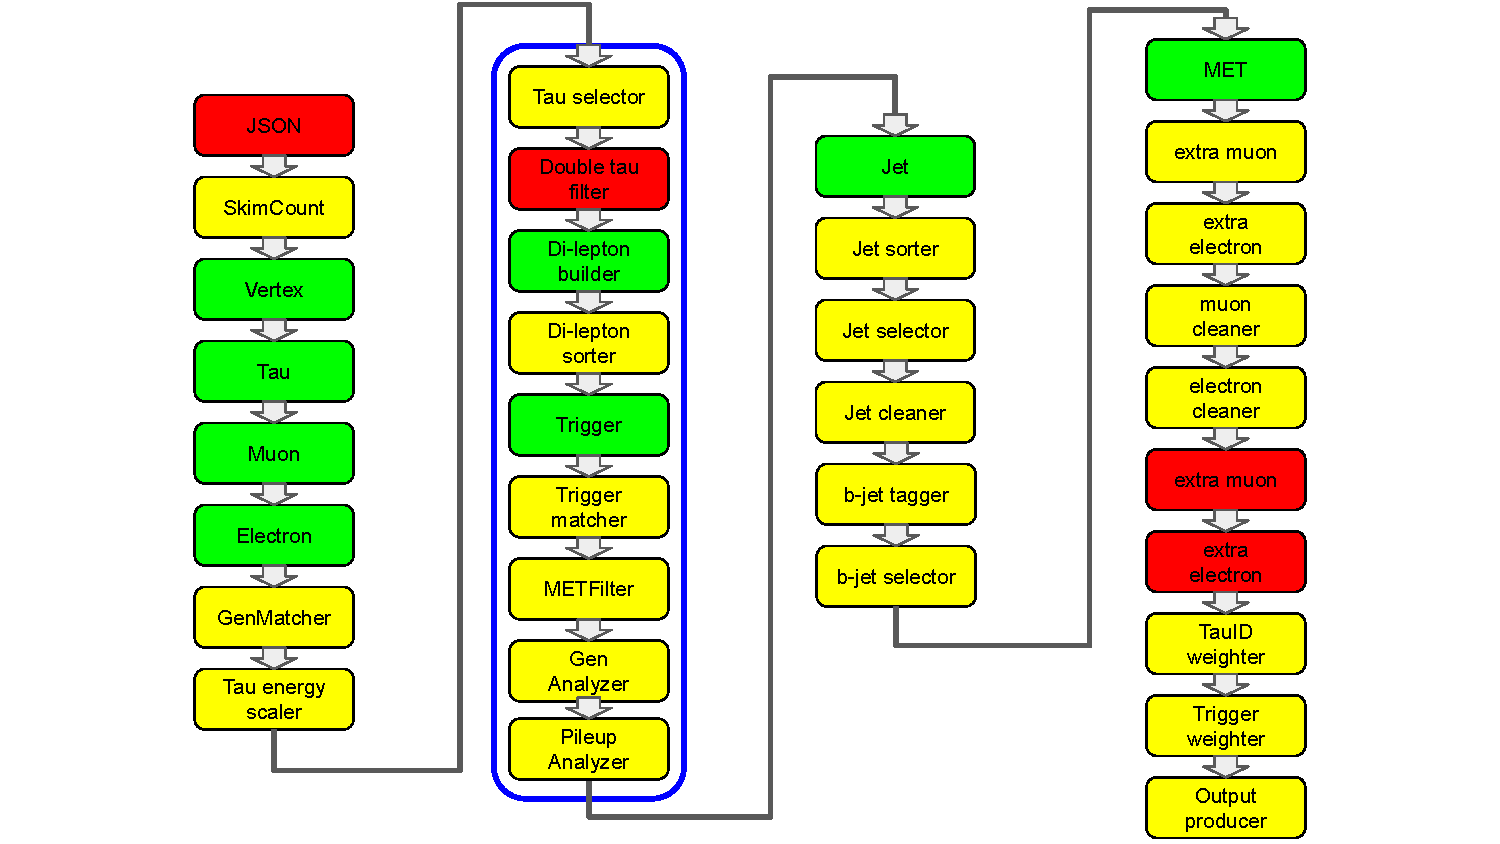
\includegraphics[width=\textwidth]{Images/HEPPY_diagram.pdf}
    \caption{Diagram of the selection flow implemented in HEPPy. Every box represents a module, called analyzer. Green analyzers create collections in the event instance by wrapping objects from the input in dedicated python classes. Yellow analyzers modify or compute a variable of the event. Red analyzers filter events, meaning if their condition is not satisfied, the chain stops, then starts again with the next event. Finally, the blue highlighted section is the only part of the sequence that is specific to the \tauh\tauh channel. The rest of the sequence is usable by other channels, like the semileptonic channels $e\tauh$ and $\mu\tauh$, and has been successfully tested.}
    \label{fig:HEPPY}
\end{figure}

HEPPy is a python event processing framework for high energy physics based on ROOT. The inputs used in this analysis follow the MINIAOD format of the CMS collaboration. This format was design to hold the event-based information needed by most analyses. Therefore, the input files hold a lot of information, i.e. the lists of reconstructed physics objects, making it quite important in size, leading to sizeable computing times. HEPPy's role is then to select events by rejecting along criteria that are defined in the next sections, while also trimming the non-analysis specific information, leading to a new light-weight format. HEPPy is an analyzer-based framework, meaning all the processing will be done in a feed-forward workflow with each step being encoded into a module called analyzer. Since most physics objects retrieved from the ROOT files will be wrapped in python classes, allowing definition of useful methods and compatibility, most analyzer of this workflow will work by manipulating the defined physics objects to either create new useful variables, select subsets of objects or reject events based on specific criteria. Most of this analysis has seen new sets of analyzers created in order to provide as much modularity and clarity as possible so that future analysis would be able to easily and promptly create this selection step. A diagram of the workflow developed in HEPPy is detailed in figure \ref{fig:HEPPY}. In order of appearance of the workflow, the role of the analyzers are: 
\begin{itemize}
    \item JSON: Only active when running on real data, rejects the events that have not been validated by the CMS collaboration.
    \item SkimCount: counts the number of simulated events pres-selections for renormalisation purposes later.
    \item Vertex/Tau/Muon/Electron: creates collection of the respective objects, wrap them in HEPPy classes, adding useful methods and attributes.
    \item Genmatcher: Only active when running on simulation, matches reconstructed hadronic taus with generator-level particles, as described in the next section.
    \item Tau energy scaler: only active when running on simulation, scales the energy of the taus, depending on their gen-level match. Stores the difference for eventual propagation to the \MET.
    \item Tau selector: first analyzer of the channel specific sequence, selects \tauh which have:
    \begin{itemize}
    \item $\pt > 40 \mathrm{GeV}$ and $|\eta| < 2.1$.
    \item Passed the PF decay mode finding discriminator detailed in section \ref{sec:std_tau_id}.
    \item $d_z$ between leading charged track and first primary vertex $d_z < 0.2 \mathrm{cm}$.
    \item Passed the very loose working point of the anti-electron discriminator and the loose working point of the anti-muon discriminator. detailed in section \ref{sec:std_tau_id}.
    \end{itemize}
    \item Double tau filter: filters the event if less than two \tauh fulfilling the requirements have been found.
    \item Di-lepton builder: creates all possible combinations of two \tauh that have passed the selections, provided:
    \begin{itemize}
    \item the pair is separated by $\Delta R > 0.5$.
    \item the pair has opposite-sign electric charges.
    \item the pair matches the trigger objects associated with one of the triggers within $\Delta R > 0.5$.
    \end{itemize}
    \item Di-lepton sorter: after those requirements there can be more than one possible candidate pair. In this case the pair with the \tauh of highest \pt is chosen. If two pairs have the same \pt for their leading \tauh, the pair which highest \pt \tauh is most isolated is chosen. If there is still two pairs, the same criteria are then used on the second \tauh.
    \item Trigger: retrieve the trigger information
    \item Trigger matcher: checks if the selected \tauh pair matches the trigger information
    \item METFilter: retireves several filters have been implemented by the CMS collaboration to reject events in order to mitigate several \MET reconstruction issues
    \item Gen analyzer: Only active when running on simulation, retrieves more generator level information in order to compute several weights, i.e the top quark and Drell-Yan \pt reweighting that are detailed in the next section.
    \item Pileup analyzer: Only active when running on simulation, retrieves pilup information and computes pileup weights, as detailed in the next section.
    \item Jet: creates collection of jets, wrap them in a HEPPy classe, adding useful methods and attributes. Also applies the jet energy corrections as detailed in next section, while also storing the information for propagation to the \MET.
    \item Jet sorter: sorts the jet collection by \pt.
    \item Jet selector: jets are required to have corrected $\pt > 30 \mathrm{GeV}$ and $|\eta| < 4.7$, and must pass identification criteria to reject fakes that originate from detector noise or pileup interactions.
    \item Jet cleaner: jets that overlap with either of the selected leptons are discarded.
    \item b-jet tagger: applies the b-tagging scheme including the promote-demote method detailed in the next section.
    \item b-jet selector: creates a b-tagged jet collection from all jets passing the b-tagging scheme and of $|\eta|<2.5$.
    \item MET: \MET focused analyzer, retrieves \MET of the event and applies all needed corrections and adjustment for previously corrected objects.
    \item extra muon(electron)/cleaners: checks the muon(electron) collections for quality criteria and rejects event with quality extra leptons, in order to avoid overlap of different channels, and to reduce background contribution.
    \item TauID/trigger weighters: compute and apply the respective correction weights detailed in the next section.
    \item Output producer: Gathers all desired retrieved/computed information and stores it in a flexible ROOT format for easy synchronisation with other analyses groups.
\end{itemize}

Indeed synchronisation at this stage is usually performed. For example a prototype of this sequence was used to synchronise with the other groups for the previous MSSM search for a heavy Higgs bosons \cite{Aaboud2018} and helped successfully figure out tweaks and upgrades in other group codes, and vice-versa. For this 2017 data analysis, a new synchronisation has been successfully performed.


\section{Background estimation methods}
\label{sec:analysis_background_methods}

For all processes apart from QCD multijets events, appropriate samples generated by MC simulation are available. In this analysis, these are still used even though in the final analysis model, a large part is described by data driven methods, which improves the data/MC agreement and reduces the involved systematic uncertainties: $\mathrm{Z} \rightarrow \tau\tau$ embedded samples replace all simulated events with two genuine tau lepton decays involved. All events where at least one of the tau candidates is faked by a jet are described by the fake factor method.

\subsection{Monte-Carlo simulation}
\label{sec:MC_corr}

Monte-carlo simulated events (MC) are meant to provide an estimation of events for processes that are not covered by the data-driven techniques. Since those techniques cover only specific parts of samples, it is necessary to be able to discern the MC events that are relevant. Therefore the reconstructed \tauh have to be matched to the generator particles available in the simulated samples. This is called generator matching. The exact definitions used for each type can be found in table \ref{tab:mc_matching}.

\begin{table}[]
    \centering
    \begin{tabular}{|c|c|l|}
        \hline
        Value & Type & Generator level object properties \\
        \hline
        1 & Prompt electron & $|\mathrm{pdgID}|==11$, $\pt > 8 \mathrm{GeV}$, status flag IsPrompt\\
        \hline
        2 & Prompt muon & $|\mathrm{pdgID}|==13$, $\pt > 8 \mathrm{GeV}$, status flag IsPrompt\\
        \hline
        3 & $\tau \rightarrow e$ & $|\mathrm{pdgID}|==11$, $\pt > 8 \mathrm{GeV}$, status flag IsDirectPromptTauDecayProduct\\
        \hline
        4 & $\tau \rightarrow \mu$ & $|\mathrm{pdgID}|==13$, $\pt > 8 \mathrm{GeV}$, status flag IsDirectPromptTauDecayProduct\\
        \hline
        5 & $\tau \rightarrow \tauh$ & Gen-tau jet \\
        \hline
        6 & Jet/pu fake & Anything that does not fall into any of the above categories \\
        \hline
    \end{tabular}
    \caption{MC generator matching}
    \label{tab:mc_matching}
\end{table}

The simulated background samples are split into three parts labeled T, J and L. T corresponds to events with gen match = 3, 4, 5 for both tau candidates. J corresponds to events with gen match = 6 for at least one of the hadronic tau candidates. L corresponds to all remaining events. In this analysis the T part of the background samples is replaced by the embedded samples and the J part is covered by the fake factor method. The remaining part is then covered by simulation.

In order to mitigate the differences between data and simulations, several measurements have provided corrections that are applied in the analysis. Which are:

\paragraph{Pileup reweighting} In order to better fit the pileup distribution in recorded data a pileup reweighting is applied to MC events to match the data distribution.

\paragraph{EE noise jets removal} Due to noise in the ECAL endcaps, all jets in the covered pseudo-rapidity of less than $50 \mathrm{GeV}$ are removed in both data and MC. The removal of the jet is also propagated to the \MET.

\paragraph{Tau ID/isolation and trigger efficiency} Data/MC scale factors (SF) measured in $\mathrm{Z}\rightarrow\tau\tau$ events with a maximum likelihood fit using the invariant mass of the tau and muon candidates as an observable are used. The SF is given for product of tau reconstruction and ID efficiency. For the embedded samples this scale factor is measured using a similar procedure. An additional correction is applied for embedded taus to correct for biases due to higher tracking efficiencies in embedded events than data. Trigger scale factors are measured using a tag and probe method. The efficiencies of the triggers are measured for data and MC and then the scale factor is computed as:
\begin{equation}
    SF = \frac{\epsilon(\mathrm{data})}{\epsilon(\mathrm{MC})} \mend
\end{equation}
The scale factors for the double-tau trigger are measured in bins of the tau \pt, $\eta$, and $\phi$. Due to a bug in the embedded samples the efficiency of the tau triggers is decreased significantly compared to the MC/data. This bug affects some of the latter HLT filters relating to the hadronic tau isolation cuts applied at HLT level. To fix this issue the embedded taus are matched to earlier filters in the HLT before the problematic part and the trigger and the scale factors are used to cover the differences. The scale factors for the embedded samples use the same $\epsilon(\mathrm{data})$ measured for the MC scale factors but use the efficiency measured for the embedded taus in the denominator, the scale factor is then computed as:
\begin{equation}
    SF = \frac{\epsilon(\mathrm{data})}{\epsilon(\mathrm{embedding})} \mend
\end{equation}

\paragraph{Tau energy scale} The tau energy scale was measured using as observables the tau mass and visible mass of the invariant system of the muon and the hadronic tau decay in $\mathrm{Z}\rightarrow\tau_{\mu}\tauh$ events. 

\paragraph{Jet energy} On top of the corrections detailed in section \ref{sec:jet_clustering}, corrections derived by the CMS collaborations are also applied \cite{collaboration_2011}.

\paragraph{Lepton to tau fake efficiency} Lepton to tau fake rates are measured by the collaboration and corrections are applied.

\paragraph{Lepton to tau fake energy scale} A correction to the central values of the \tauh energies for \tauh candidates originating from electron (muon) fakes is applied for the 1-prong and 1-prong+1-\pizero decay-modes. 

\paragraph{Recoil corrections} Recoil corrections are applied to correct for the mismodeling of \MET in the simulated samples of Drell-Yan, W+Jets and Higgs production. The corrections are measured in $\mathrm{Z} \rightarrow \mu\mu$ events and performed on the variable defined as the vectorial difference of the measured missing transverse momentum and total transverse momentum of neutrinos originating from the decay of Z, W or Higgs boson. The corrections are propagated to \MET using
\begin{equation}
    \Vec{U} = \Vec{\MET} - \Vec{p}_{T,\nu} \mend
\end{equation}

\paragraph{Top quark transverse momentum reweighting} The modeling of the $t\Bar{t}$ background is improved by reweighting the \pt spectrum of the top quarks.

\paragraph{b-tagging efficiency} The efficiency for the tagging of b jets and the mistagging rate for light-flavour jets has been measured in both data and simulation. Differences are corrected for in the simulation through the application of efficiency and mistagging scale factors. The values of these factors and a description of the methods used to determine them can be found in \cite{Sirunyan_2018}. The simulation is corrected by randomly reclassifying a fraction of tagged jets as non-tagged, or vice versa, as necessary to result in the correct average efficiency. The promotion or demotion probabilities for each jet are defined as
\begin{equation*}
    P(\mathrm{demote}) = 1 - SF \msep when SF < 1
\end{equation*}
\begin{equation*}
    P(\mathrm{promote}) = \frac{(SF-1)F}{\frac{SF}{\epsilon-1}} \msep when SF > 1 \mend
\end{equation*}
The scale factors, $SF$, are $\pt$, $\eta$ and jet-flavour dependant ratios of data and simulation efficiencies, and $\epsilon$ is the tagging efficiency in simulation.

\subsection{Hybrid Data-Monte-Carlo estimation : embedding}

The embedding technique allows an estimation of the genuine $\tau\tau$ standard model backgrounds from data, with minimal simulation input. In the data, the muons are removed from reconstructed $\mu\mu$ events and replaced with simulated tau leptons with the same kinematic properties. In that way a set of hybrid events is obtained that relies on simulation only for the decay of the tau leptons. challenges in describing the underlying event or the production of associated jets in the simulation are avoided. A detailed description of the embedding technique can be found in \cite{CMS:2018apv}.

In this analysis, embedded samples are used and replace the MC simulated samples for $\mathrm{Z}\rightarrow \tau\tau$ and the parts of $t\Bar{t}$, di-boson and electroweak events where both tau candidates match to genuine taus at generator level.

\subsection{Data-driven estimation : fake factor method}

The fake factor method (FF) can be used to predict all background sources with gluon- or quark-initiated jets misidentified as hadronic $\tau$ decays. The method is based on measuring two numbers: the number of events where jets pass the nominal \tauh identification (ID) criteria (called isolated), corresponding to the signal region selection of the corresponding analysis, and the number of events where jets satisfy a set of loose ID criteria, but fail the nominal \tauh ID criteria (inverted isolation, referred to as “anti-isolated” in the following). The FF is defined as the ratio of the two numbers:
\begin{equation}
    FF = \frac{\text{passes preselection and passes MVA-based \tauh ID discriminant WP}}{\text{passes preselection and fails MVA-based \tauh ID discriminant WP}}
\end{equation}
and is applied as a weight to events which pass the corresponding signal region selection except that the events are required to contain \tauh candidates satisfying the loose preselection criteria, but failing the nominal \tauh ID criteria (application region). The fake factor is estimated as a function of the jet multiplicity (0 or $\geq$ 1). The \pt dependency is fit. This is done separately for the QCD multi-jet, the W+jets and the $t\Bar{t}$ background.

The fake factors are also determined separately for each of the channels $e\tauh$, $\mu\tauh$, and $\tauh\tauh$, accounting for differences in the selected background composition, the trigger requirements and in the \tauh ID criteria applied in each channel. Considered candidates have to pass a set of common requirements, which are the same in each channel, and channel-specific cuts on the MVA-based \tauh ID discriminant and on the discriminants against electrons and muons. The common requirements include passing the $\tauh$ decay mode reconstruction and satisfying the conditions $\pt > 23 \mathrm{GeV}$ and $|\eta| < 2.3$. Furthermore, candidates are required to pass the very–loose working point of the MVA-based \tauh ID discriminant. The discriminants against electrons and muons that are applied are identical to the discriminants against electrons and muons that are applied on the level of the nominal \tauh ID criteria for a given channel.

For the \tauh\tauh channel, the determination region requirement is that the electric charges of the two hadronic $\tau$ candidates have the same sign. As for this channel the multi-jet background is by far the dominant fake background, the fake factors measured in the QCD determination region are also used to estimate any other backgrounds.

The fake factor applied to a given event in the application region is a weighted average of the values measured in the three control regions. The weight is given by the expected fraction of events of a given type in the application region. The weight is binned in $m_{vis}$ and number of jets for inclusive distributions. This weighted fake factor is applied to all events in this region. From the resulting distribution, the expected contribution from events with actual hadronic $\tau$ decays are subtracted using simulation. The expected fraction of events is estimated in two independent ways: via a template fit to the observed data, and via simulation. As the results of both methods agree and the template fit has convergence problems in some low-statistics event categories, the simulation-based estimate is used.

\section{Systematic uncertainties}
\label{sec:analysis_systematics}

This section describes the sources of uncertainty that affect the signal and background predictions of the \mttot distributions. The experimental uncertainties typically concern either object selection or the methods to estimate the backgrounds described in the previous section, and are inherent to their respective measurement. The object selection are more important for the signal prediction, whereas the estimation methods have a large effect on the background estimation. Theoretical uncertainties affect the predictions of both signal and background but are larger for the signal. Most uncertainties affect only the rate of signal, but a smaller number may affect both the shape and rate. Throughout this section the values of uncertainties given as percentages refer directly to variations in the predicted signal and background yields, unless otherwise specified.

\subsection{Shape uncertainties}
The following uncertainties cause variations in the shapes of the process templates which are realized via event-wise application of the respective shifts.

\paragraph{Tau energy scale} Shape uncertainties are applied for each decay mode. In the embedded samples we have hybrid events where the simulated taus might be mixed with calorimeter deposits remaining from the muon cleaning. For this reason, the tau energy scale uncertainties for embedded samples are split into two parts where $50\%$ are fully correlated with the uncertainty for fully simulated samples and $50\%$ are uncorrelated.

\paragraph{Jet energy scale} In general, the CMS collaboration derives uncertainties on the jet energy scale from 28 sources and combines them in a single uncertainty with one nuisance parameter. This uncertainty has turned out to be overconstrained in the previous analysis and during the preparations of this analysis. For this reason the uncertainty is split into several parts, not to all 27 sources, because this would result in a large technical effort. Instead, the sources are grouped according to the affected detector regions.

\paragraph{Lepton to \tauh fake energy scale} Uncertainty shifts are applied to the \pt of lepton to \tauh fakes in MC samples uncorrelated between decay modes.

\paragraph{\MET unclustered energy uncertainty} The \MET unclustered energy uncertainty is applied to all MC processes that do not have recoil correction applied.

\paragraph{\MET recoil correction uncertainties} For all MC processes that have recoil correction, uncertainties determined by varying the hadronic response and its resolution within the uncertainties determined during the computation of the recoil corrections.

\paragraph{Top \pt reweighting} Uncertainty between no and twice the correction on the re-weighting applied to $t\Bar{t}$ events.

\paragraph{DY \pt reweighting} Uncertainty of $10\%$ of the correction on the re-weighting applied to $\mathrm{Z}\rightarrow ll$ events.

\paragraph{B-tagging efficiency} The uncertainties from the b-tagging scale-factors provided by the CMS collaboration are propagated to the shapes.

\paragraph{\tauh tracking efficiency in embedding} An uncertainty on the tracking efficiency of hadronic taus in the embedded samples is propagated uncorrelated between 1 and 3 prong decay modes.

\paragraph{Fake-factor uncertainties} Uncertainties on the $j \rightarrow \tauh$ templates consist of several sources:
\begin{itemize}
    \item Statistical uncertainty of the fake factor measurement in the control regions, given by the fit uncertainty to the \pt dependence.
    \item Systematic uncertainties related to the multi-jet fake factor corrections. The uncertainties are added in quadrature for each channel individually:
    \begin{itemize}
        \item Uncertainty of the non-closure correction, as a function of the visible mass.
        \item Uncertainty on the \pt of the other hadronic $\tau$ candidate.
        \item Uncertainty on the correction function for the extrapolation from the SS to the OS region.
    \end{itemize}
    \item Systematic uncertainties on the fraction of W/Z+jets events and $t\Bar{t}$ events with one misidentified \tauh in the AR, adding two nuisance parameters. This is evaluated by varying the fractions of each background within uncertainties (including cross section and experimental uncertainties), while readjusting the fractions of the other processes to keep the sum at $100\%$.
\end{itemize}

\paragraph{Bin-by-bin uncertainties} To account for statistical shape uncertainties in the backgrounds due to the use of Monte-Carlo and embedded samples or templates derived from data events with limited number of events, we introduce shape variations to the background templates in all categories following the Barlow-Beeston approach, where the statistical uncertainties on each bin are used to define alternative shapes.

\subsection{Normalization uncertainties}
The following uncertainties are applied as log normal uncertainties on the yield of the affected
processes.

\paragraph{Luminosity} $2.3 \%$ luminosity uncertainty is applied to the templates which originate from MC simulation \cite{CMS:2018elu}.

\paragraph{Tau ID efficiency} The uncertainty is applied to all processes where the yield is estimated from MC. Since two hadronic taus are required in the \tauh\tauh channel the magnitude of correlated and uncorrelated uncertainty is $5.5\%$ respectively $2.4\%$. For the embedded samples the same uncertainties on the tau ID SF are taken. The embedded samples also have an additional uncertainty applied to cover a tracking efficiency correction, this is determined by taking the weighted average of the uncertainties on the tracking corrections and has a magnitude of $2\%$ (per-tau).

\paragraph{Trigger efficiency} The uncertainty on the trigger efficiencies amounts to $10\%$. The uncertainty is applied to all processes where the yield is estimated from MC and to the embedded samples. The embedded and MC uncertainties are uncorrelated. An additional $4\%$ uncertainty ($2\%$ per muon $= 4\%$) is applied to embedded samples in order to take account of efficiency of the double muon trigger that was used to select input events for the embedding technique.

\paragraph{Background normalization uncertainty} A $4\%$, $5\%$, $6\%$ and $4\%$ uncertainty is applied to the $Z\rightarrow ll$, di-boson/single top, $t\Bar{t}$ and EWKZ processes respectively to account for the uncertainty on the production cross section. 

\paragraph{Lepton to tau fake rate} Shape uncertainties were checked and no significant shape dependency has been observed in the event distributions used in this analysis. Therefore log normal uncertainties of $16\%$ ($26\%$) are applied for electron (muon) to tau fake rate.

\paragraph{Fake factor normalization} The uncertainty due to the subtraction of the genuine tau contribution in the anti-isolated AR. This is estimated by varying the genuine-tau yield by $\pm 10\%$, and amounts to about $2\%$. The fake factor shape uncertainties are normalized to the same area as the nominal shape, and the normalization factors are added in quadrature and act as separate nuisance parameters: this is done separately for the statistical uncertainties on the raw fake factors (about $5\%$) and the systematic uncertainties on the corrections (about $7\%$). Uncertainties are split in shape(-only) and yield uncertainties to capture the main variations induced by the uncertainties. This describes the two leading degrees of freedom of the fake factor \pt fits evaluated by toy experiments.

\section{Statistical interpretation}
\label{sec:analysis_statistical_interpretation}

This section outlines the statistical procedure used to quantify or reject the presence of a signal in data. These methods were developed by the LHC Higgs Combination Group to provide a common strategy for both the CMS and ATLAS Collaborations and to facilitate the combination of individual search results \cite{CMS-NOTE-2011-005}. 

The expected Higgs boson event yields in a given model can be denoted as $s$ and the expectations from background as $b$. This can refer equally to single event counts, or to predicted binned distributions for use in a shape-based analysis. An additional factor $\mu$ is introduced as a signal strength modifier, which allows for models to scale the signal rate as $\mu \times s$. The background-only hypothesis is therefore defined by $\mu = 0$, and any signal hypothesis by $\mu > 0$. The term "data" will refer to a corresponding observed event count or counts, which could originate from an actual experiment or from simulation. The yields $s$ and $b$ are, in general, functions of some parameters $\theta$ representing experimental and theoretical uncertainties: $s(\theta)$ and $b(\theta)$. The nominal values $\Tilde{\theta}$ of these nuisance parameters are usually determined by external measurements, with uncertainties described by probability density functions $p(\Tilde{\theta} | \theta)$. From these components the likelihood for an observed dataset, $\Lagr(\mathrm{data}|\mu,\theta)$, is defined as
\begin{equation}
    \Lagr(\mathrm{data}|\mu,\theta) = \mathrm{Poisson}(\mathrm{data}|\mu\times s(\theta) + b(\theta)) \times p(\Tilde{\theta}|\theta) \msep
\end{equation}
where for a binned likelihood model the Poisson tern is simply the product of Poisson probabilities over each bin $i$:
\begin{equation}
    \mathrm{Poisson}(\mathrm{data}|\mu\times s(\theta) + b(\theta)) = \prod_{i} \frac{(\mu s_i + b_i)^{n_i}}{n_i !} e^{-\mu s_i -b_i} \mend
\end{equation}

A ratio of likelihoods can be used to define a test statistic, a single number which can distinguish between two hypotheses. Such a test statistic can be used to set upper limits on the rate of signal production. Historically, a number of definitions have been used in Higgs boson searches. The one chosen by the LHC experiments is known as the profile likelihood ratio
\begin{equation}
    q_{\mu} = -2 \mathrm{ln}\frac{\Lagr(\mathrm{data}| \mu, \Hat{\theta}_{\mu})}{\Lagr(\mathrm{data}|\Hat{\mu},\Hat{\theta})} \text{, with the constraint } 0\leq \Hat{\mu}\leq \mu \msep
\end{equation}
where $\mu$ is the signal hypothesis being tested; $\Hat{\theta}_{\mu}$ are the values of the nuisance parameters that maximise the likelihood, given the fixed signal strength $\mu$; and $\Hat{\mu}$ and $\Hat{\theta}$ are the values which give the global maximum of the likelihood. The constraint $0\leq\Hat{\mu}$ is added to prevent an unphysical negative signal strength. The constraint $\Hat{\mu}\leq\mu$ is chosen to prevent the exclusion of any $\mu$ lower than the best fit $\Hat{\mu}$, thus ensuring the construction of a one-sided confidence interval. Large values of $q_{\mu}$ indicate a value of $\mu$ that the data disagrees with, whereas values close to zero indicate good compatibility with the signal hypothesis in question. The probability of finding a value $q_{\mu}$ at least as large as the observed value, $q_{\mu}^{\mathrm{obs}}$, is defined as
\begin{equation}
    \label{eq:cl}
    \mathrm{CL}_{s+b} = \int^{inf}_{q_{\mu}^{\mathrm{obs}}} f(q_{\mu}|\mu,\Hat{\theta}_{\mu})dq_{\mu} \msep
\end{equation}
where $f(q_{\mu}|\mu,\Hat{\theta}_{\mu})$ is the probability distribution function for $q_{\mu}$. The tested value of $\mu$ is then said to be excluded at a confidence level $\alpha$, where $\alpha = 1 - \mathrm{CL}_{s+b}$. The $95\%$ CL is typically chosen when setting upper limits. One issue with this definition is that in some cases it will lead to the exclusion of low signal strengths, where an analysis may not expect to have sensitivity. For example, this may happen with a downward fluctuation of the data where the signal expectation is very small compared to the background expectation. To protect against this, an additional probability $\mathrm{CL}_b$ can be introduced, defined similarly to equation \ref{eq:cl}, but under the assumption of the background-only hypothesis, $f(q_{\mu}|0,\Hat{\theta}_0)$. Instead, the ratio of these probabilities, denoted $\mathrm{CL}_s$, where
\begin{equation}
    \mathrm{CL}_s = \frac{\mathrm{CL}_{s+b}}{\mathrm{CL}_b}\msep
\end{equation}
is used to set the $95\%$ CL exclusion limit, and this is commonly referred to as the modified frequentist approach \cite{Read_2002}.

The distributions $f(q_{\mu}|\mu,\Hat{\theta}_{\mu})$ and $f(q_{\mu}|0,\Hat{\theta}_0)$ can be determined by generating toy MC datasets from their respective models, in which the nuisance parameters are fixed to the values found in the fits to the observed data. The value of $q_{\mu}$ is then determined for each toy dataset. The effect of systematic uncertainties is incorporated by sampling a set of pseudo-measurements $\Tilde{\theta}$ in each toy using the chosen nuisance pdfs. It is often instructive to compare the observed exclusion limit to the expectation under the assumption of the background-only hypothesis. This can be determined by generating background-only toy datasets and determining the $95\%$ CL limit in each. These values form a cumulative pdf from which the median exclusion and uncertainty bands can be extracted.

A profile likelihood ratio can also be used to calculate the p-value for an observed excess of events given the background-only hypothesis. For this a slightly modified definition of the test statistic is required,
\begin{equation}
    q_0 = -2 \mathrm{ln}\frac{\Lagr(data|0, \Hat{\theta}_0)}{\Lagr(data|\Hat{\mu}, \Hat{\theta}}, \text{ with the constraint }\Hat{\mu} \geq 0\msep 
\end{equation}
where the constraint $\Hat{\mu} \geq 0$ is chosen to prevent a downward fluctuation being consideres evidence against the background-only hypothesis. The p-value for the observed data is then given as
\begin{equation}
    p_0 = \lim^{\inf}_{q_o^{\mathrm{obs}}} f(q_0 | 0, \Hat{\theta}_0) dq_0\msep
\end{equation}
where $f(q_0 | 0, \Hat{\theta}_0)$ can be determined by generating pseudo-data from the background-only hypothesis. The p-value is typically converted to a significance, Z, by determining the number of standard deviations of a one-sided normal distribution that would yield an equal tail probability.

A major advantage of the profile likelihood test statistic is that in the limit of a large data sample, the distribution $f(q_{\mu})$ follows a known formula \cite{Carena2013}. This so-called asymptotic limit approximation removes the need for the computationally intensive step of generating and fitting toy datasets, which can take an appreciable time for models with many bins and nuisance parameters. This method relies on the properties of the Asimov dataset, a single representative dataset in which the observed rates match exactly with the prediction of the model under the nominal set of nuisance parameters. Furthermore, it is possible to derive a formula for the median expected limit and uncertainty bands using only the properties of the Asimov dataset, thus completely removing the need for any toy MC \cite{Carena2013}.

\section{Results and interpretations}
\label{sec:analysis_results}

